\documentclass{article}

\usepackage{graphicx}
\usepackage{tikz}
\usepackage{tikzsymbols}
\usetikzlibrary{calc,patterns,shapes.geometric}
\pagestyle{empty}
\usepackage[margin=0pt]{geometry}
\geometry{papersize={14in,12in}}

\def\centerarc[#1](#2)(#3:#4:#5){\draw[#1] ($(#2)+({#5*cos(#3)},{#5*sin(#3)})$) arc (#3:#4:#5);}

\begin{document}
	\begin{figure}
		\centering
		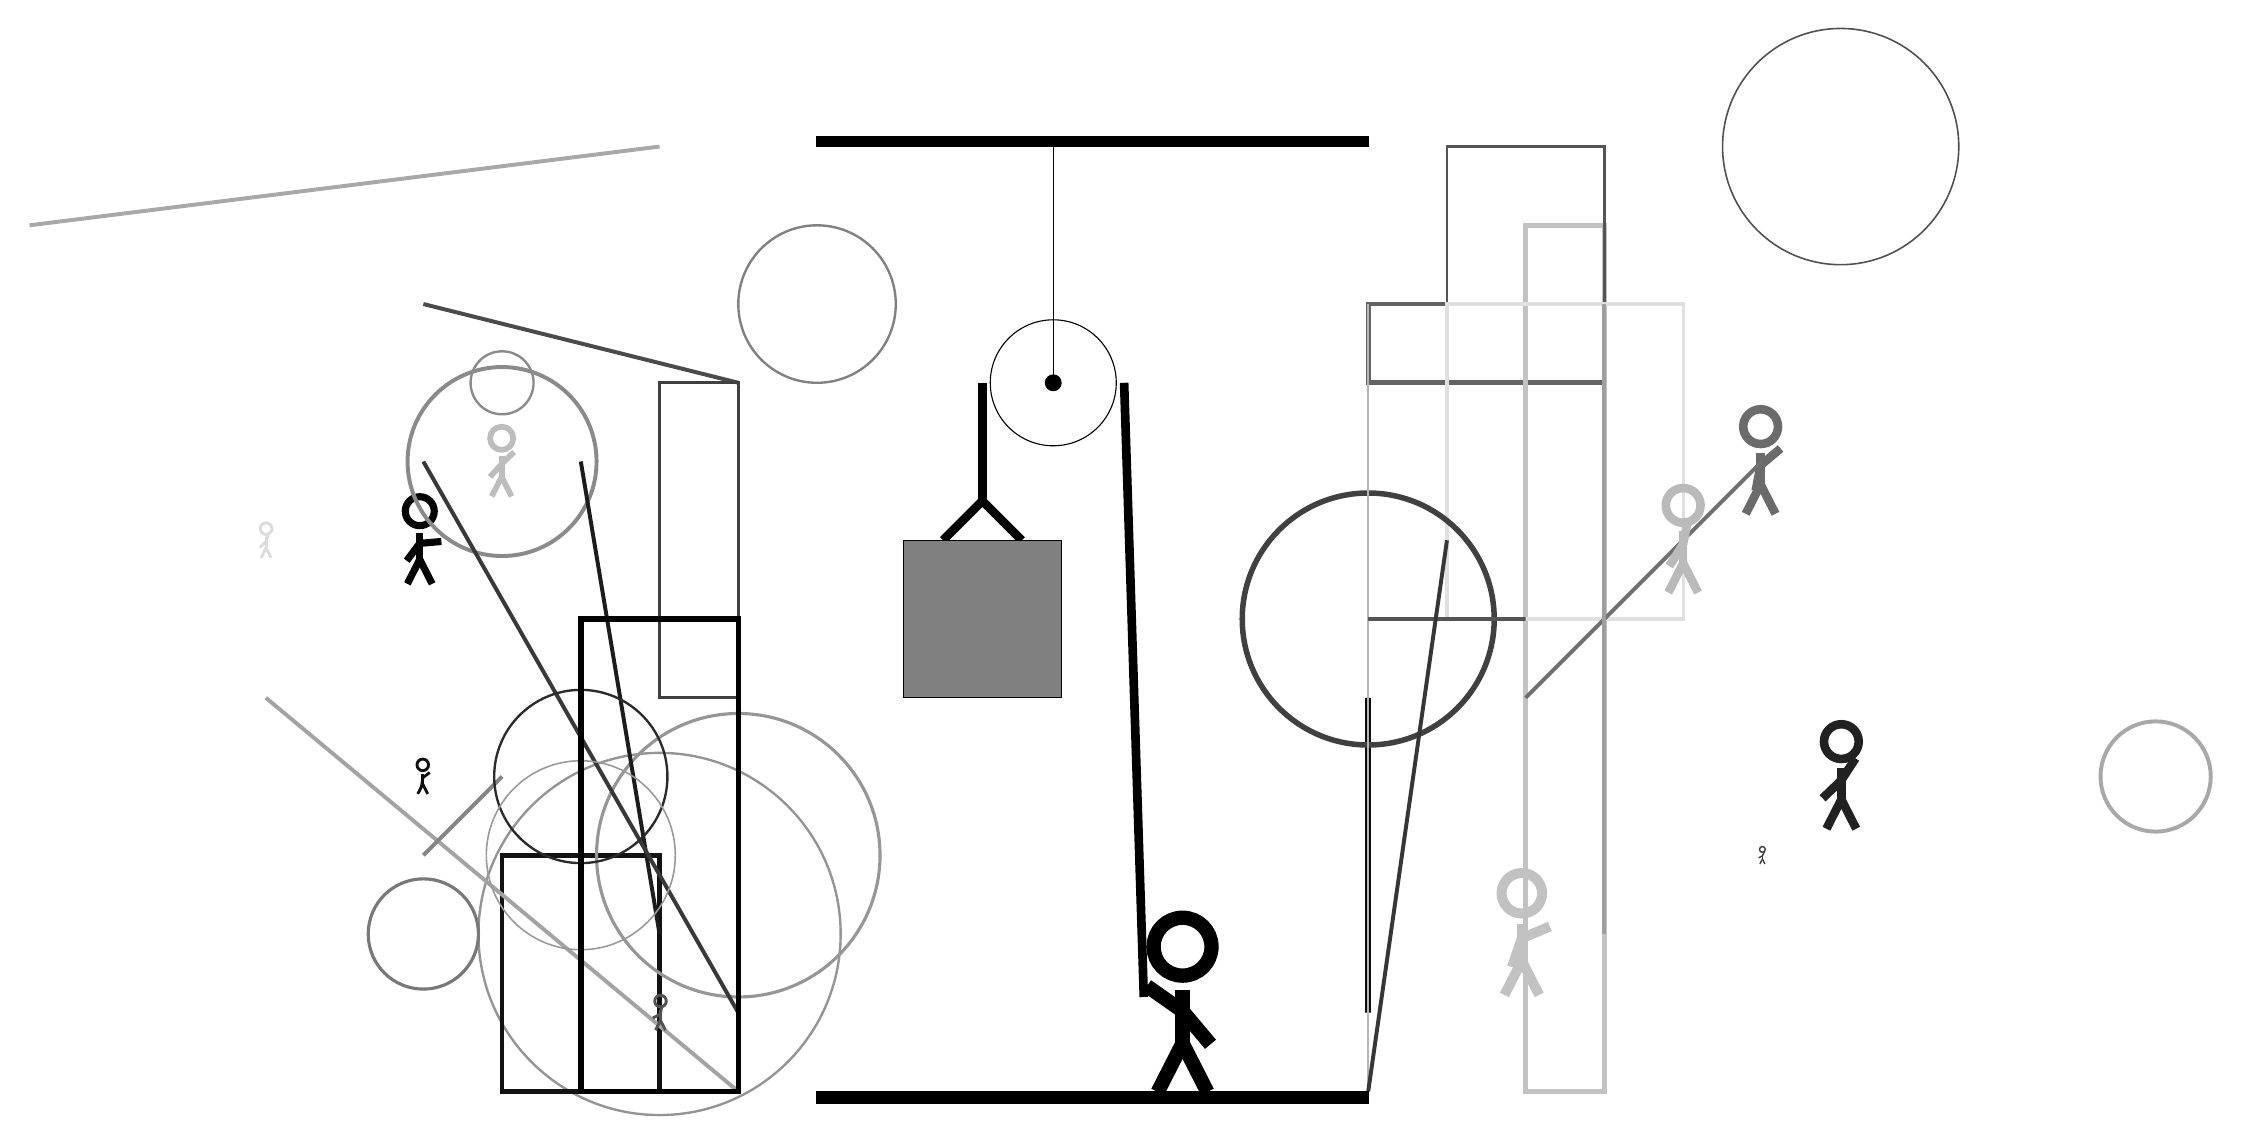
\begin{tikzpicture}
			%%%%% START %%%%%
			
			\draw[fill=black] (-2, 9) rectangle (5, 9.125);
			
			\draw (1, 6) circle (0.8);
			\draw[fill=black] (1, 6) circle (0.1);
			\draw (1, 9) -- (1, 6);
			
			\draw[line width=1.1mm] (-0.4, 4.0) -- (0.1, 4.5) -- (0.6, 4.0);
			\draw[fill=black!50] (-0.9, 4.0) rectangle (1.1, 2.0);
			
			\draw[line width=1.1mm] (0.1, 6) -- (0.1, 4.5);
			\centerarc[line width=1.1mm](1, 6)(0:180:0.9);
			\draw[line width=1.1mm](1.9, 6) -- (2.15, -1.8);
			
			\node at (2.6, -1.9) {\Strichmaxerl[10][-35][-50]};
			
			\node[line width=0.6mm, color=black!98] at (-7, 4) {\Strichmaxerl[5][53][5]};
			
			\draw[line width=0.6mm, color=black!61] (5, 6) rectangle (8, 7);
			\node[line width=0.6mm, color=black!24] at (7, -1) {\Strichmaxerl[7][71][23]};
			\draw [line width=0.3mm, color=black!46](-6, 6) circle (0.4);
			\draw[line width=0.7mm, color=black!24] (7, 8) rectangle (8, -3);
			\draw [line width=0.5mm, color=black!46](-6, 5) circle (1.2);
			\draw[line width=0.5mm, color=black!34](-4, 9) -- (-12, 8);
			\node[line width=0.6mm, color=black!95] at (-7, 1) {\Strichmaxerl[2][82][37]};
			\draw[line width=0.3mm, color=black!67] (6, 7) rectangle (8, 9);
			\node[line width=0.7mm, color=black!58] at (10, 5) {\Strichmaxerl[6][79][40]};
			\draw[line width=0.5mm, color=black!71](-3, 6) -- (-7, 7);
			
			\draw[line width=0.4mm, color=black!12] (6, 7) rectangle (9, 3);
			\draw [line width=0.3mm, color=black!42](-4, -1) circle (2.3);
			
			\node[line width=0.3mm, color=black!87] at (11, 1) {\Strichmaxerl[6][44][57]};
			\draw [line width=0.3mm, color=black!50](-2, 7) circle (1.0);
			\node[line width=0.3mm, color=black!75] at (10, 0) {\Strichmaxerl[1][27][64]};
			
			\draw[line width=0.6mm, color=black!93] (-4, -3) rectangle (-6, 0);
			
			\draw [line width=0.4mm, color=black!41](-3, 0) circle (1.8);
			\draw[line width=0.5mm, color=black!56](10, 5) -- (7, 2);
			\draw[line width=0.7mm, color=black!96] (5, -2) rectangle (5, 2);
			\draw[line width=0.5mm, color=black!89](-4, -1) -- (-5, 5);
			
			\draw[line width=0.4mm, color=black!75] (-3, 6) rectangle (-4, 2);
			
			\draw [line width=0.7mm, color=black!75](5, 3) circle (1.6);
			\draw[line width=0.5mm, color=black!78](-7, 5) -- (-3, -2);
			\draw [line width=0.2mm, color=black!69](11, 9) circle (1.5);
			\draw[line width=0.5mm, color=black!36](-3, -3) -- (-9, 2);
			\node[line width=0.3mm, color=black!68] at (-4, -2) {\Strichmaxerl[2][28][81]};
			\draw[line width=0.5mm, color=black!48](-7, 0) -- (-6, 1);
			\node[line width=0.5mm, color=black!26] at (-6, 5) {\Strichmaxerl[4][48][44]};
			\draw [line width=0.3mm, color=black!83](-5, 1) circle (1.1);
			\draw[line width=0.3mm, color=black!29] (5, 7) rectangle (5, -3);
			\draw [line width=0.5mm, color=black!34](15, 1) circle (0.7);
			\draw[line width=0.6mm, color=black!67] (7, 3) rectangle (5, 3);
			\draw [line width=0.4mm, color=black!53](-7, -1) circle (0.7);
			\node[line width=0.2mm, color=black!27] at (9, 4) {\Strichmaxerl[6][58][79]};
			\draw [line width=0.2mm, color=black!40](-5, 0) circle (1.2);
			
			\draw[line width=0.5mm, color=black!38](8, -1) -- (8, 7);
			
			\node[line width=0.7mm, color=black!14] at (-9, 4) {\Strichmaxerl[2][44][75]};
			\draw[line width=0.7mm, color=black!100] (-3, -3) rectangle (-5, 3);
			\draw[line width=0.5mm, color=black!79](6, 4) -- (5, -3);
			
			\draw[fill=black] (-2, -3) rectangle (5, -3.15);
			
			%%%%% END %%%%%
		\end{tikzpicture}
	\end{figure}	
\end{document}